\documentclass{article}
\usepackage[a4paper, total={6in, 9in}]{geometry}
\usepackage{array,multirow,graphicx}
\usepackage{float}
\usepackage{multicol}

\usepackage{hyperref}
\hypersetup{
    colorlinks=true,
    linkcolor=blue,
    filecolor=magenta,      
    urlcolor=cyan,
}

\newcommand{\STAB}[1]{\begin{tabular}{@{}c@{}}#1\end{tabular}}
\graphicspath{ {./} }

\title{
    Speechify - Implementation\\
    \begin{large}
        Winter 2021 - COMM 302 - Assignment 4
    \end{large}
}
\author{Jamie Won - 20113217}

% lifetime for saas = retention

% Channels of Marketing
% Viral marketing
% Public Relations
% Unconventional PR
% Search Engine Marketing -> Google search ads -> Moment of intent -> If searching for google, probably want it
% Social & display ads 
% Offline ads
% Search Engine Optimization -> oonoly 10\% youtube users actually click ad -> Rest click natural results -> Identify key words
% Content Marketing
% Email Marketing
% Engineering as Marketing
% Targeting Blog
% Business development
% Sales
% Affiliate Programs
% Existing Platforms
% Trade Shows
% Offline EvangelistsSpeaking Engagements
% Community Building

% Growth Hacking

\begin{document}
\maketitle
\vfill
It should be noted that this assignment was based on a template from: Aulet B (2017): Disciplined Entrepreneurship Workbook. Whiley and sons, New Jersey
\cleardoublepage
\tableofcontents
\cleardoublepage

\section{Map The Process to Acquire a Paying Customer}
    \subsection{Qualitative summary}
    The process to acquire a paying customer involves identifying leads, considering suspected potential users, engaging prospective users and finally stimulating the purchasing intent for qualified prospects. In order to continue earning after the initial purchase, customer loyalty must be assured through customer satisfaction and for further promotion, these satisfied customers will be Speechify's advocate amongst their peers.

    Of the action plans listed above, the ones with most confidence are customer advocacy and loyalty. Whereas, the action plan of least confidence is stimulating purchase intent. The following subsection details the action plans for each step in the customer acquisition process.
    \subsection{Action Plans}
        \begin{figure}[h!]
            \begin{center}
                
                \begin{tabular}{| p{4.2cm} | p{9cm} |}
                    \hline
                    \textbf{Type} & \textbf{Action Plan} \\
                    \hline
                    Identification $\rightarrow$ Leads & Take advantage of search engine marketing and optimization to figure out who users are; become an in-kind sponsor to hackathons, and see who uses Speechify, and the types of hacks made  \\
                    \hline
                    Consideration $\rightarrow$ Suspects & Target people in the music, video editting, content creator industry and purchase ads in commonly used software for these users; become an in-kind sponsor for competitions for products/services that Speechify was most used for in hackathons (previous stage)  \\
                    \hline
                    Engagement $\rightarrow$ Prospects & Put user stories and feedback on marketing material, ensure that this is easily located; continue narrowing down users; create interactive demos / marketing materials to identified segments \\
                    \hline
                    Purchase Intent $\rightarrow$ Qualified Prospects & Create a sense of urgency by having a discount available only for a limited time, or the same thing but with paid features; If there are amazing existing projects that have used Speechify, contact their creator, ask for feedback, their story and permission to use it for marketing \\
                    \hline
                    Purchase $\rightarrow$ Customers & Offer discounted first months and free trials for premium features; use numbers to describe the time saved by existing users (or if none, estimated time saved) \\
                    \hline
                    Loyalty $\rightarrow$ Satisfied Customers & Ensure that the product is everything described and more (NOT less); offer discounts based on user type to sweeten the deal, particularly near the time of resubscription. \\
                    \hline
                    Advocacy $\rightarrow$ Evangelists & Offer promotions for [successful] referrals; create a platform that allows this to be done easily; consistently improve/add features or integration to existing software so that there is always "more" for existing users to talk about with peers\\
                    \hline
                \end{tabular}
                \caption{Table depicting action plans for each stage of the customer acquisition process.}
            \end{center}
            \end{figure}

\section{Estimate TAM for next Markets}
    \begin{multicols}{2}
        \raggedright \textbf{Beachhead Market}: Content Creators\\
        \textbf{Follow-On Markets}:
        \begin{enumerate}
            \item Content Creators (Beachhead Market)
            \item Video Editors
            \item Audiobook Companies
            \item Music Writing Platforms
            \item Authors
            \item Educational Institutions
        \end{enumerate}
            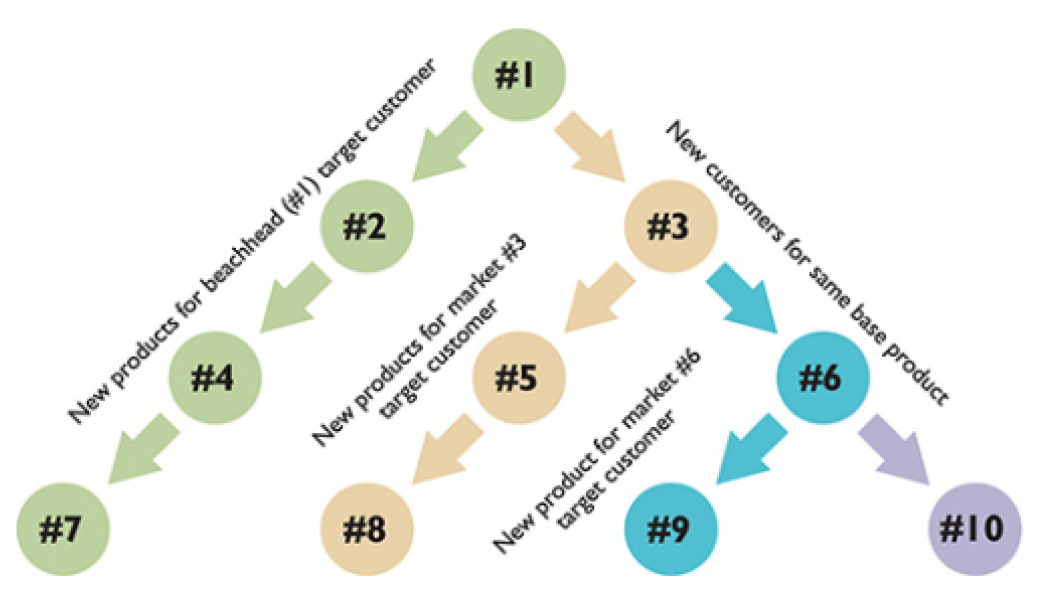
\includegraphics[width=7cm, height=6cm]{TAMGraph}
            \par{Image from the worksheet detailing which market in the list to the left is an "adjacent" or "additional" market}
    \end{multicols}
    \begin{figure}[h!]
        \begin{center}
            \begin{tabular}{| p{2.5cm} | p{1.6cm} | p{3.5cm} | p{3.65cm} | p{1.1cm} | c |}
                \hline
                \raggedright \textbf{Candidate \& Same Product Customer} &
                    \raggedright \textbf{How it leverages your Core} &
                    \raggedright \textbf{Pros of selling to this market} & 
                    \raggedright \textbf{Cons of selling to this market} & 
                    \raggedright \textbf{TAM est. (\$)} & 
                    \multirow{3}{*}{\STAB{\rotatebox[origin=c]{90}{\textbf{Rank}}}}
                \\ \hline
                \raggedright Content Creators - Beachhead & 
                    \raggedright Save time; generate more; Enhance content &
                    \raggedright Speechify is targeted to this market (see previous assignments) &
                    \raggedright Very diverse market & 
                    720000 & 1
                \\ \hline
                \raggedright Video Editors - Same Customer & 
                    \raggedright Saves time; generate more &
                    \raggedright Massive need; Large market; Tiered users & 
                    \raggedright Difficult to position; competition & 
                    500000 & 2
                \\ \hline
                \raggedright Audiobook Companies - Same Product & 
                    \raggedright Earn more from existing product &
                    \raggedright Will not need to modify product much & 
                    \raggedright Targeting organization instead of individual; may have legal red tape & 550000 & 3
                \\ \hline
                \raggedright Music Writing Platforms - Same Customer & 
                    \raggedright Saves time; generate more &
                    \raggedright If successful, niche market & 
                    \raggedright Not all writers do it digitally; many platforms to integrate with; small market & 50000 & 6
                \\ \hline
                \raggedright Authors - Same Customer & 
                    \raggedright Earn more from existing product&
                    \raggedright Minimal product modification; potential growth; easier to target than companies & 
                    \raggedright Small market; wrong demographic (age); needs different features; limited need & 600000 & 5
                \\ \hline
                \raggedright Educational Institutions - Same Product & 
                    \raggedright Enhance content &
                    \raggedright Lengthy contracts; some student licencees are future users; enhances learning and teaching experience & 
                    \raggedright Targeting organization instead of individual; will have legal red tape & 300000 & 4
                \\ \hline
            \end{tabular}
            \caption{Summary of Follow-On TAM Estimate and Priorities}
        \end{center}
    \end{figure}

    \begin{figure}[h!]
        \begin{center}
            \begin{tabular}{| p{1.9cm} | p{1.5cm} | p{1.6cm} | p{1.1cm} | p{1.25cm} | p{5cm} |}
                \hline
                \raggedright \textbf{Candidate Name} &
                    \raggedright \textbf{Est. \# of Users} & 
                    \raggedright \textbf{Est. Yearly Revenue Per User} & 
                    \raggedright \textbf{Est. TAM Range} & 
                    \raggedright \textbf{Est. CAGR (\%)} &
                    \textbf{Other Considerations (Profitability, time to conquer, potential market share, investment required, competition, etc)} 
                \\ \hline
                \raggedright Content Creators & 50000 & 60 & 70000 - 100000 & 4.6 & beachhead market; likely easiest to penetrate
                \\ \hline
                \raggedright Video Editors & 25000 & 60 & 35000 - 50000 & 5.8 & subset of content creators; will need to tailor integrations for existing platforms
                \\ \hline
                \raggedright Audiobook Companies & 5 & 10000 & 25000 - 60000 & 5.9 & competitors exist
                \\ \hline
                \raggedright Music Writing Platforms & 10 & 3000 & 20000 - 50000 & 2.8 & primary research must be conducted to determine if this is viable
                \\ \hline
                \raggedright Authors & 10000 & 60 & 40000 - 70000 & .5 & competitors exist; should be easier to target than organizations
                \\ \hline
                \raggedright Educational Institutions & 100 & 10000 & 70000 - 120000 & 2.7 & having institutions purchase a license will be difficult but profitable
                \\ \hline
            \end{tabular}
            \caption{Individual Worksheet for Follow-On Market Segment}
        \end{center}
    \end{figure}

\section{LTV}
    \subsection{One Time Charge(s)}
        \subsubsection{What will your one-time charges be for each customer?}
        Individual users: \$60; Medium enterprises: \$3000; Large enterprises: \$10000

        \subsubsection{What is your estimated profit margin on your one-time charges?}
        This is a SAAS product thus, the idea of a profit margin per one-time charge isn't the most accurate or even feasible measure. Assuming yearly subscriptons of \$60 for basic features, and about \$20000 to make the basic product, Speechify will break even at 334 subscriptions.

        \subsubsection{What is the life of the product before a customer has to reppurchase the product?}

        1 year. However, if longer contracts are negotiated, that is with educational institutions for example, then it would be for the duration of the contract.

        \subsubsection{What percentage of customers will repurchase?}
        
        About 50\%. Students in institutions without a license will need it for 4 years. Dropouts won't. Bloggers and vloggers will renew it if they do well.

        \subsubsection{What will your recurring revenue streams be?}

        Same as repurchase - the renewing of subscriptions.

        \subsubsection{What is your profit margin on your recurring revenue streams?}

        Please see section 3.12

        \subsubsection{What is the retention rate for your recurring revenue streams?}
        
        Please see section 3.13 and below
        \begin{itemize}
            \begin{multicols}{2}
                \item After first/second year: 50\%
                \item After third year: 45\%
                \item After fourth year: 40\%
                \item After fifth year: 45\%
            \end{multicols}
        \end{itemize}
        These numbers are based on several assumptions and facts:
        \begin{itemize}
            \item Fact: there is currently no product on the market like Speechify
            \item Assumption: it will take around 2 years for competitors to develop a competing product
            \item Assumption: Speechify will have a strong brand name by the end of the first year
            \item Assumption (Goal): Speechify will sign a license with a large institution by latest, midway through the second year
            \item Assumption: As other competitors enter the market, Speechify may lose some customers, but also steal others that have been attracted by competitor products.
        \end{itemize} 

        \subsubsection{What other revenue sources will you have? What will your profit margin be, and is there a yearly retention rate applicable to them?}

        Ad-free usage or banner ads on the main website. These should cancel out the fees for posting advertisements of its own. There is no applicable yearly retention rate.

        \subsubsection{What will your cost of capital be, and why?} 
        Unknown - Assumed 50\% as per instructions

    \subsection{Calculations to Estimate the LTV}
        \begin{figure}[ht!]
            \begin{center}
                \begin{tabular}{| p{6.5cm} | c | c | c | c | c | c |}
                    \hline
                    \textbf{Input} & \textbf{t=0} & \textbf{t=1} & \textbf{t=2} & \textbf{t=3} & \textbf{t=4} & \textbf{t=5}
                    \\ \hline
                    \textbf{A.} One-time revenue amount & 50 & 60 & 60 & 60 & 60 &60  
                    \\ \hline
                    \textbf{B.} One-time revenue profit margin (\%) $^{1}$ & -- & -- & -- & -- & -- & -- 
                    \\ \hline
                    \textbf{C.} One-time revenue profit (row A*B) $^{2}$ & 50 & 60 & 60 & 60 & 60 &60  
                    \\ \hline
                    \textbf{D.} Recurring revenue amount & 0 & 60 & 60 & 60 & 60 &60  
                    \\ \hline
                    \textbf{E.} Recurring revenue profit margin (\%) $^{1}$ & -- & -- & -- & -- & -- & -- 
                    \\ \hline
                    \textbf{F.} Recurring revenue profit (row D*E) $^{3}$& 0 & 30 & 30 & 27 & 24 & 27
                    \\ \hline
                    \textbf{G.} Other revenue amount & 0 & 0 & 0 & 0 & 0 & 0
                    \\ \hline
                    \textbf{H.} Other revenue profit margin (\%) $^{1}$ & -- & -- & -- & -- & -- & -- 
                    \\ \hline
                    \textbf{I.} Other revenue profit (row G*H) & 0 & 0 & 0 & 0 & 0 & 0
                    \\ \hline
                    \textbf{J.} Sum of profit for time period & 60 & 90 & 90 & 87 & 84 & 87
                    \\ \hline
                    \raggedright \textbf{K.} Default cost of capital factor: Discount factor to NPV (@ 50\%/year and assuming of time = years) & 1.0 & .67 & .44 & .30 & .20 & .13
                    \\ \hline
                    \textbf{L.} NPV of each item (row J*K) & 60 & 60.3 & 39.6 & 26.1 & 16.8 & 12.6
                    \\ \hline
                    \textbf{M.} Sum of all NPVS (sum of all cells in row L) & --- & \multicolumn{4}{c}{215.4} &
                    \\ \hline
                    
                \end{tabular}
                \caption{Table depicting the calculated LTV estimates. It should be noted that 't' refers to a time from today in years, and the revenue is that in CAD.}
            \end{center}
        \end{figure}
        
        \raggedright
        [1] Note that Speechify is an SAAS product and thus, unit margins are not a useful calculation

        [2] These values are the one time fee

        [3] This is the one time fee multiplied by the retention rate (simple not compound)

    \subsection{Interpretation of Estimation}

        \subsubsection{What would you round your LTV estimation to? What range do you feel comfortable with?}

        250K. Not only was it calculated simply (as opposed to compounded), this value was rounded down. Speechify aims to err on the side of caution. 

        \subsubsection{Where do you feel the bigest unknowns are in your LTV estimation calculation?}

        Profit margins per unit. This is simply not possible to calculate due to the nature of the product. I estimate that the initial year and a half of revenue should go into costs for development, investments, marketing and research (about 96K) from research into other SAAS models. This results in it being about 150K.

        \subsubsection{Does the number seem reasonable?}

        Yes. It's conservative, but for 5 years, seems appropriate.

        \subsubsection{What are the key drivers of the LTV if you want to increase it?}

        Four key drivers were considered: Cross-Selling \& Up-Selling, Customer Advocacy \& Referrals, Repeat Purchases/Renewals and the cost to serve. The cost to serve will be constant - a site to host and distribute the product, and thus, not a major factor in increasing the LTV. Cross-Selling \% Up-Selling and Repeat Purchases/Renewals are the key drivers to Speechify's LTV. The previous section mapped out potential markets for expansion and the profit within. Speechify hopes to have retentioon rates of 50\%, which is a major part of the revenue stream, and the factor: Repeat Purchases/Renewals. Advocacy/Referrals will also increase the LTV, but those come with having a reliable product (which also causes the other two situations)

        \subsubsection{Where do you think you have the greatest opportunity to increase LTV, all things considered?}

        With repeat purchases/renewals. Speechify's base product and any subsequent expansions, integrations or features will cost a significant amount to build, but nothing outside of site hosting to resell. Any subscription renewal for the same product is thus arguably worth more for Speechify.

    \section{COCA}

        \subsection{Assumptions for COCA Estimation}
        
            \textbf{What time intervals did you define for the following phases in the Step 18 worksheet "Sales Channels for the Short, Medium and Long Term"?}

            Short Term: 1 year
            
            Medium Term: 3 years
            
            Long Term: 5 years

        \subsection{Total Sales and Marketing Expenses List}

            List the expected sales and marketing expenses, and their costs, This input will be used when estimating the COCA.

            \begin{figure} [h!]
                \begin{center}
                    \begin{tabular}{| p{2.75cm} | p{3.5cm} | p{3.5cm} | p{3.5cm} |}
                        \hline
                        \textbf{Sales Expenses} & \textbf{Short Term} & \textbf{Medium Term} & \textbf{Long Term}
                        \\ \hline
                        & 10K & 15K & 15K
                        \\ \hline
                        \raggedright \textbf{Marketing Expenses} &
                            \raggedright \textbf{Short Term} & 
                            \raggedright\textbf{Medium Term} & \textbf{Long Term}
                        \\ \hline
                        & 25K & 23K & 20K
                        \\ \hline
                    \end{tabular}
                    \caption{A table depicting the estimated expenses over the three time periods}
                \end{center}
            \end{figure}
            Research shows that depending on the type of SAAS, significantly more money is spent on Marketing than Sales, and that it ranges from 30-35\% of the ARR each year.

        \subsection{Estimate the COCA}

        \begin{figure} [h!]
            \begin{center}
                \begin{tabular}{| p{6cm} | c | c | c | c | c |}
                    \hline
                    & \textbf{Year 1} & \textbf{Year 2} & \textbf{Year 3} & \textbf{Year 4} & \textbf{Year 5}
                    \\ \hline
                    \textbf{New customers forecasted} & 1200 & 2000 & 2500 & 2800 & 3000
                    \\ \hline
                    \textbf{All sales expenses for period} & 10K & 15K & 15K & 15K & 15K 
                    \\ \hline
                    \textbf{All marketing expenses for period} & 25K & 23K & 23K & 23K & 20K
                    \\ \hline
                    \raggedright \textbf{Total marketing and sales expenses for period} & 35K & 38K & 38K & 38K & 35K
                    \\ \hline
                    \textbf{COCA for the period} & 29.1 & 19 & 15.2 & 13.6 & 11.6
                    \\ \hline
                \end{tabular}
            \end{center}
        \end{figure}
    
    \subsection{Convert Estimation into Short, Medium and Long Term Ranges}

        Short-term: \$20 - 35; Medium-term: \$15 - 25; Long-term (steady state): \$7 - 15 

    \subsection{Key Drivers of COCA and ways to Decrease It}

    \begin{figure}[h!]
        \begin{center}
            \begin{tabular}{| c | p{2cm} | c | p{3.5cm} | p{5cm} |}
                \hline
                \raggedright \textbf{\#} &
                    \raggedright \textbf{Item} &
                    \raggedright \textbf{Effect} &
                    \raggedright \textbf{Action Possible to Decrease} & 
                    \textbf{Risk}
                \\ \hline
                \textbf{1} & \raggedright Hackathon &  Medium & \raggedright Decrease cash prizes, keep platform usage for the weekend & Short Term: High (no inclination for use without incentive); Long Term: low (strong branding)
                \\ \hline
                \textbf{2} & \raggedright Advertising Budget & High & \raggedright Create advocates from a reliable product & Short term: High; Long term: Low (need and having branding)
                \\ \hline
                \textbf{3} & \raggedright Distribution Platform Development Budget & Medium & \raggedright Decrease it in the future, allowing enough for maintenance & Short term: High - proper development is a good investment; Long term: Low (only maintenance is needed)
                \\ \hline
                \textbf{4} & \raggedright Renewal Promotions & Medium & \raggedright Lower as years pass & Medium (all terms) - people may choose to not resubscribe
                \\ \hline
                \textbf{5} & Trade Shows & Low & Don't do these & No risk as trade shows are not for SAAS products
                \\ \hline
            \end{tabular}
            \caption{A table detailing key COCA drivers and how to decrease it}
        \end{center}
    \end{figure}

    \subsection{Comparison of LTV and COCA over Time}
    \begin{figure}
        \begin{center}
            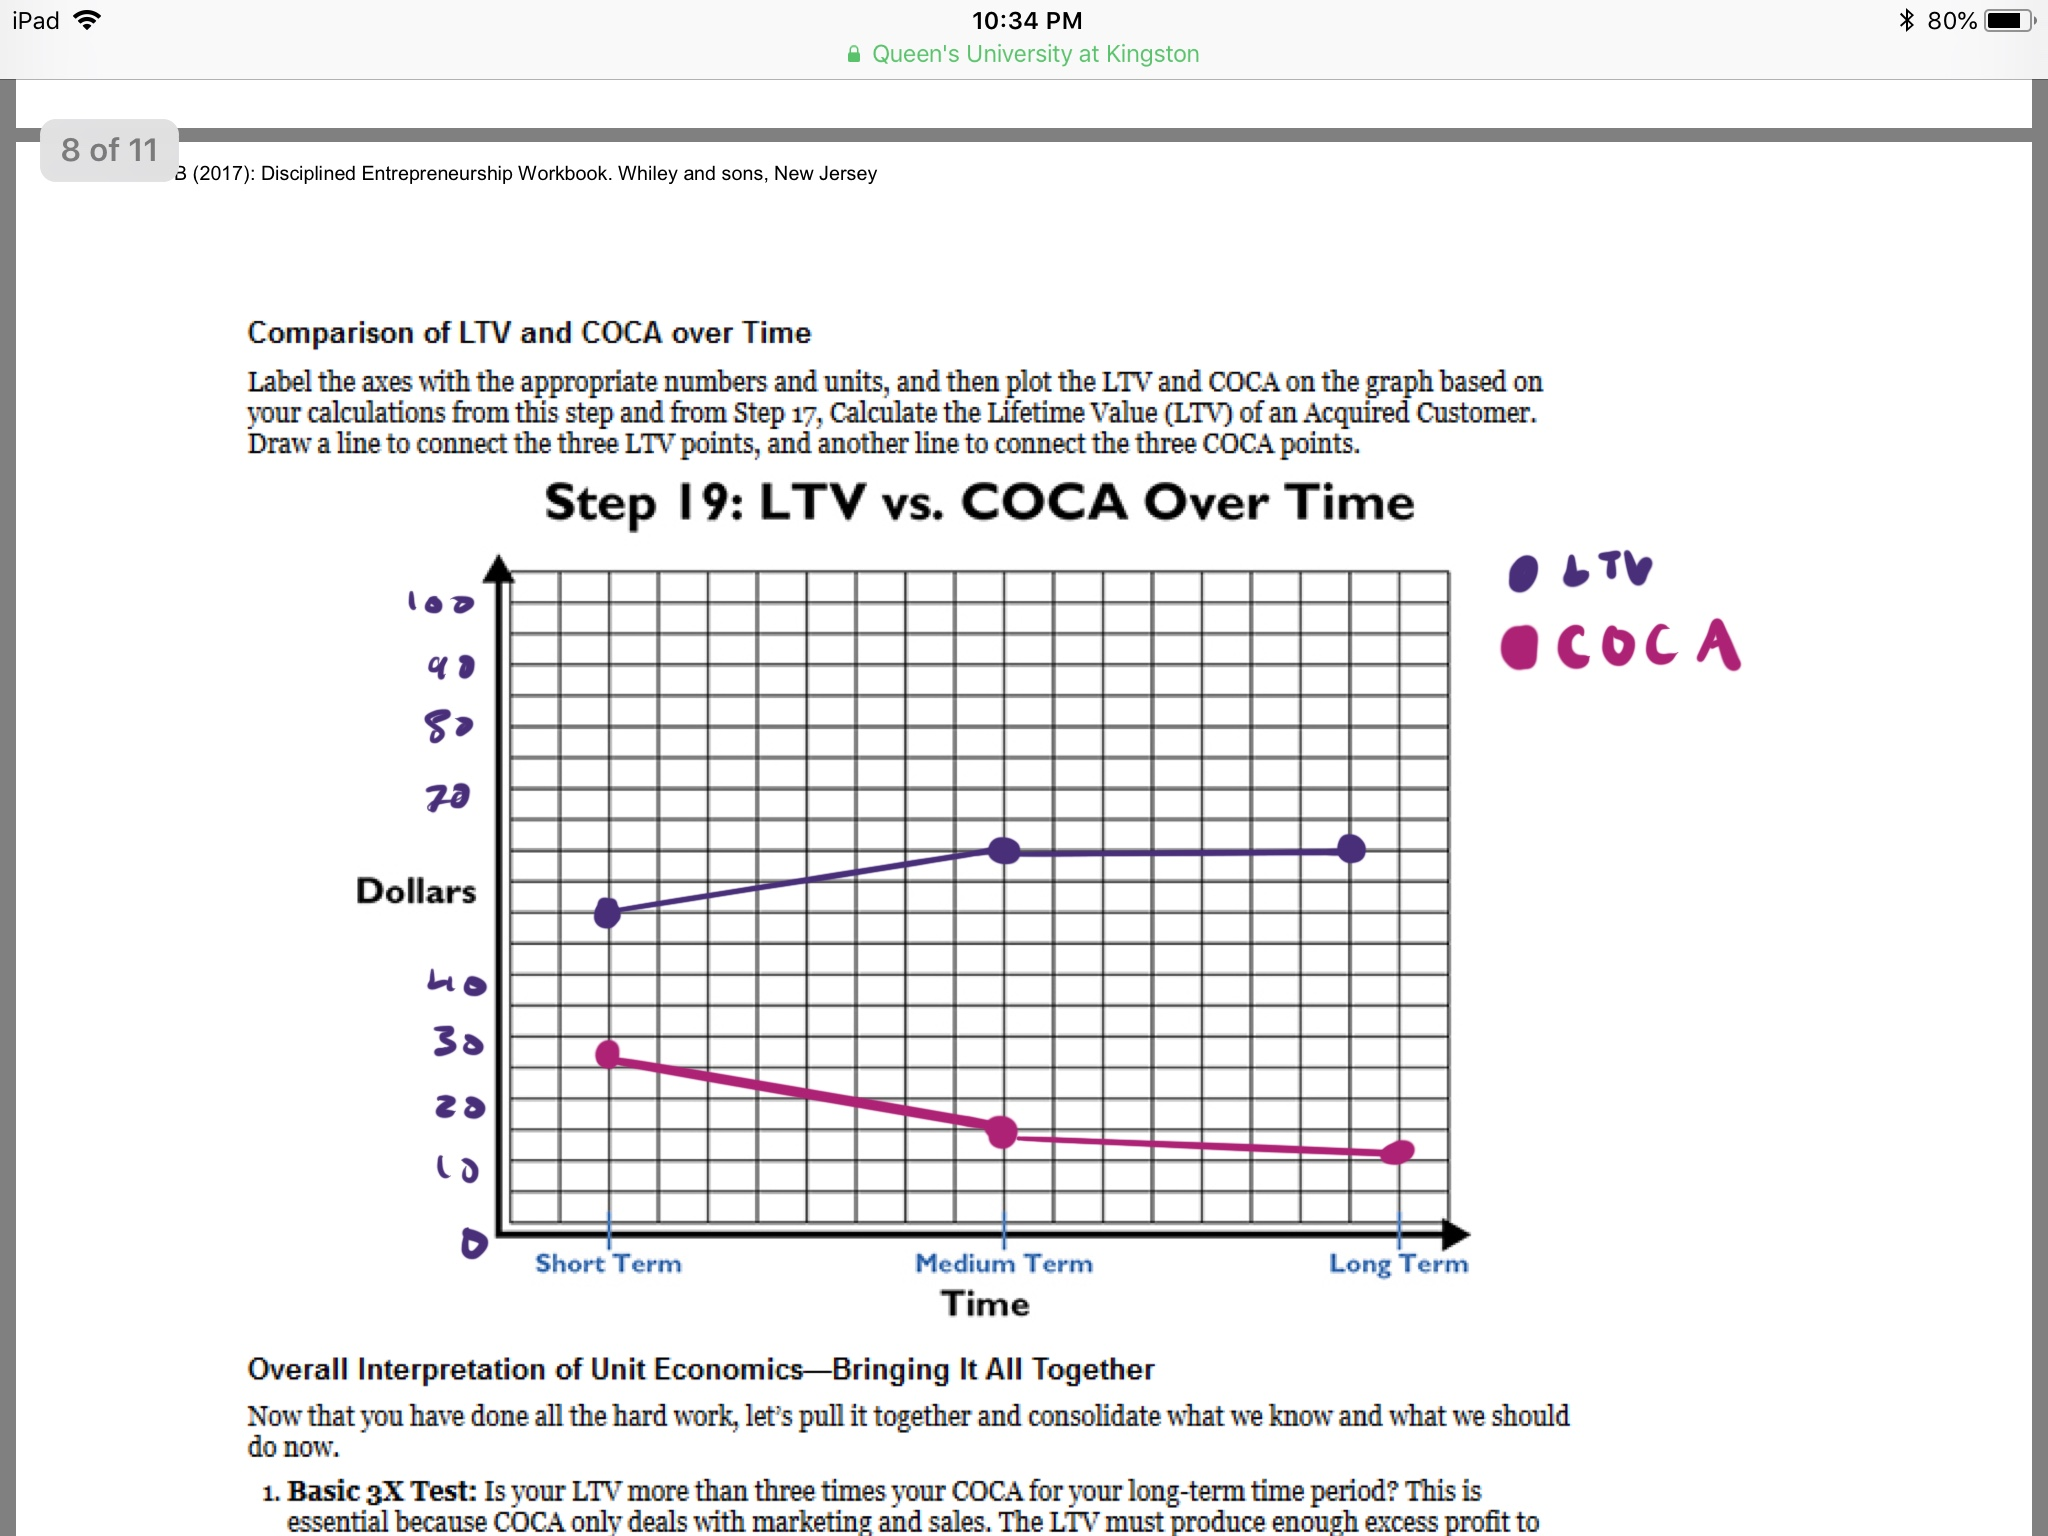
\includegraphics[width=12cm, height=6cm]{LTVCOCA}
            \caption{An image showing the comparison of the LTV and COCA. Due to some technical issues, it could not be cropped better}
        \end{center}
    \end{figure}
    \subsection{Overall Interpretation of Unit Economics}
        \subsubsection{Basic 3X Test}
        The LTV is 3x more than the COCA. It clears it by a reasonable amount.
        \subsubsection{R\&D Factor}
        The R\&D Factor should be the same as an average SAAS company, that is, some testers, integrated software specialists and a team of developers will be needed, as with other SAAS companies.

\section{Develop a product plan/roadmap}
    
    \subsection{Product Plan - Version 2 for the Beachhead Market}
    \begin{figure}[h!]
        \begin{center}
            \begin{tabular}{ | c | p{2.5cm} | p{3.5cm} | p{2.5cm} | p{2.3cm} | c |}
                \hline
                \raggedright \textbf{\#} &
                    \raggedright \textbf{Feature / Function} &
                    \raggedright \textbf{Benefit} &
                    \raggedright \textbf{How does it leverage your Core?} & \raggedright \textbf{Estimated Resources needed to develop} & \textbf{Priority} 
                \\ \hline
                \textbf{1} & Text analysis & Uses S.A. & Boosts efficiency & \$10K & High
                \\ \hline
                \textbf{2} & Audio analysis & \raggedright Further leverages S.A. & Boosts efficiency & \$1K & High
                \\ \hline
                \textbf{3} & Image analysis & \raggedright Further leverages S.A. & Boosts efficiency & \$1K & Low 
                \\ \hline
                \textbf{4} & \raggedright Build your own music & Tiered users & \raggedright Custom content & \$10K & Low
                \\ \hline
                \textbf{5} & Tiered tunes & Tiered Users & \raggedright Custom Content & \$10K & Medium
                \\ \hline
                \textbf{6} & \raggedright Software Integration - video & \raggedright Complementary product = more users & Ease of use & \raggedright Depends on software & Medium
                \\ \hline
            \end{tabular}
            \caption{Product Plan - Version 2 for the Beachhead Market}
        \end{center} 
    \end{figure}

    \subsection{Product Plan - Version 3 for the Beachhead Market}
        \begin{figure}[h!]
            \begin{center}
                \begin{tabular}{ | c | p{1.75cm} | p{2.5cm} | p{1.25cm} | p{2cm} | p{2cm} | c |}
                    \hline
                    \raggedright \textbf{\#} &
                        \raggedright \textbf{Feature / Function} &
                        \raggedright \textbf{Benefit} &
                        \raggedright \textbf{For Whom} &
                        \raggedright \textbf{How does it leverage your Core?} &
                        \raggedright \textbf{Estimated Resources needed to develop} &
                        \textbf{Priority}
                    \\ \hline
                    \textbf{1} & \raggedright Software Integration - Audio recording & \raggedright Complementary product = more users & \raggedright End User & \raggedright Ease of use & 10K & Medium
                    \\ \hline
                    \textbf{2} & \raggedright License bundling - Large & \raggedright Sold to larger institutions & \raggedright End User & \raggedright efficiency in creation & 3K & High
                    \\ \hline
                    \textbf{3} & \raggedright License bundling - Small & \raggedright Sold to small businesses & \raggedright End User & \raggedright efficiency in creation & 500 & High
                    \\ \hline
                    \textbf{4} & \raggedright License bundling - medium & \raggedright Sold to medium businesses & \raggedright End User & \raggedright efficiency in creation & 1K & High
                    \\ \hline
                    \textbf{5} & \raggedright Suggestion for music composition & \raggedright Attract customers & \raggedright End User & \raggedright New Content & 10K & Low
                    \\ \hline
                    \textbf{6} & \raggedright Software Integration - Image Selection & \raggedright Complementary product = more users & \raggedright End User & \raggedright Ease of Use & 10K & Medium
                    \\ \hline
                \end{tabular}
                \caption{Product Plan - Version 3 for the Beachhead Market}
            \end{center} 
        \end{figure}

        It ought to be noted that many of the features detailed in Figure 8 and Figure 9 would also be used by follow-up market operators. It should also be noted that Video Editors are a subset of Content Creators (see previous assignment). However, the ones being targeted in the beachhead market are the young professionals. The follow-up market for video editors refers to industry professionals and teams.

    \subsection{Other Activities beyong the functionality for the Beachhead Market}
        \begin{enumerate}
            \item Offer referral bonuses. It will be similar to the EQ Bank system, where each successful referral rewards the referrer with some amount of money. This value increases for subsequent referrals before reaching a cap.
            \item Research additional target segments. This process was outlined earlier, but is essential to see if there are better customers, and if so, how to access them. However, focus will primarily be on acquiring customers from the selected segment, as infrastructure is already there, and to retain existing customers, as they are worth "more" per renewal as with the nature of SAAS products.
            \item Find a PR team that attends hackathons/innovation challenges and gicves speeches. This is essential for raising awareness of the product and for enticing future users.
        \end{enumerate}

    \subsection{Moving Beyond the Beachhead Market - Analysis and Prioritization of Follow-On Market Candidates}
        The following table is rotated 90 degrees from the one given in the worksheet to allow for better information display
        \begin{figure}[h!]
            \begin{center}
                \begin{tabular} { | p{1.75cm} | p{2cm} | p{2cm} | p{2cm} | p{2cm} | p{2cm} |}
                    \hline
                    \textbf{\# / Field} & 1 & 2 & 3 & 4 & 5
                    \\ \hline
                    \textbf{Name} & \raggedright Video Editors & \raggedright Audiobook Companies & \raggedright Music Writing Platforms & \raggedright Authors & \raggedright Educational Institutions
                    \tabularnewline \hline
                    \raggedright \textbf{Which market does it follow from} & \raggedright Content Creators & \raggedright Content Creators & \raggedright Video Editors & \raggedright AudioBook Companies & \raggedright Content Creators 
                    \tabularnewline \hline
                    \textbf{Pros} & \raggedright Need is present; Video Editting softwares are similar - ease of integration & \raggedright Same Product & \raggedright Niche market - success means recurring subscriptions & \raggedright Matches mission - help creators get more value for their time & \raggedright Chance of large, recurring revenue 
                    \tabularnewline \hline
                    \textbf{Cons} & \raggedright Integration is difficult or restricted for each software; May have legal tape & \raggedright Negotiating with an organization is difficult; "Companies" are usually individuals that host work on major sites & \raggedright No guaranteed need at all; alternatives exist (do it manually) & \raggedright Difficult to reach out to each operator individually, will require a distribution platform & \raggedright Guaranteed legal red tape; Has potential to ruin brand if there is a mistake in version released
                    \tabularnewline \hline
                    \raggedright \textbf{Does it leverage your core?} & Yes & Yes & No & Yes & Yes
                    \tabularnewline \hline
                    \textbf{Priority} & High & Medium & Low & Low & Medium
                    \tabularnewline \hline
                    \raggedright \textbf{Key factors needed to succeed} & \raggedright Audio and text analysis; Integration software & \raggedright Audio and text analysis; Successful negotiation & \raggedright Software negotiation; Sheet music analysis; Strong promotion & \raggedright Strong promotion; Distribution channel; Text analysis & \raggedright Strong negotiation; Bundling; Basic product
                    \tabularnewline \hline
                    \raggedright \textbf{Required Resources} & \multicolumn{5}{l}{Due to the nature of the service, this was combined with the previous row} 
                    \tabularnewline \hline
                    \textbf{Risk} & Low & Medium & High & High & Medium 
                    \tabularnewline \hline
                    \textbf{Reward} & High & Medium & Low & Medium & Hgih 
                    \tabularnewline \hline
                \end{tabular}
            \end{center}
            \caption{Moving Beyond the Beachhead Market - Analysis and Prioritization of Follow-On Market Candidates}
        \end{figure}
    
    \subsection{Product Plan Overview}
    \begin{figure}[h!]
        \begin{center}
            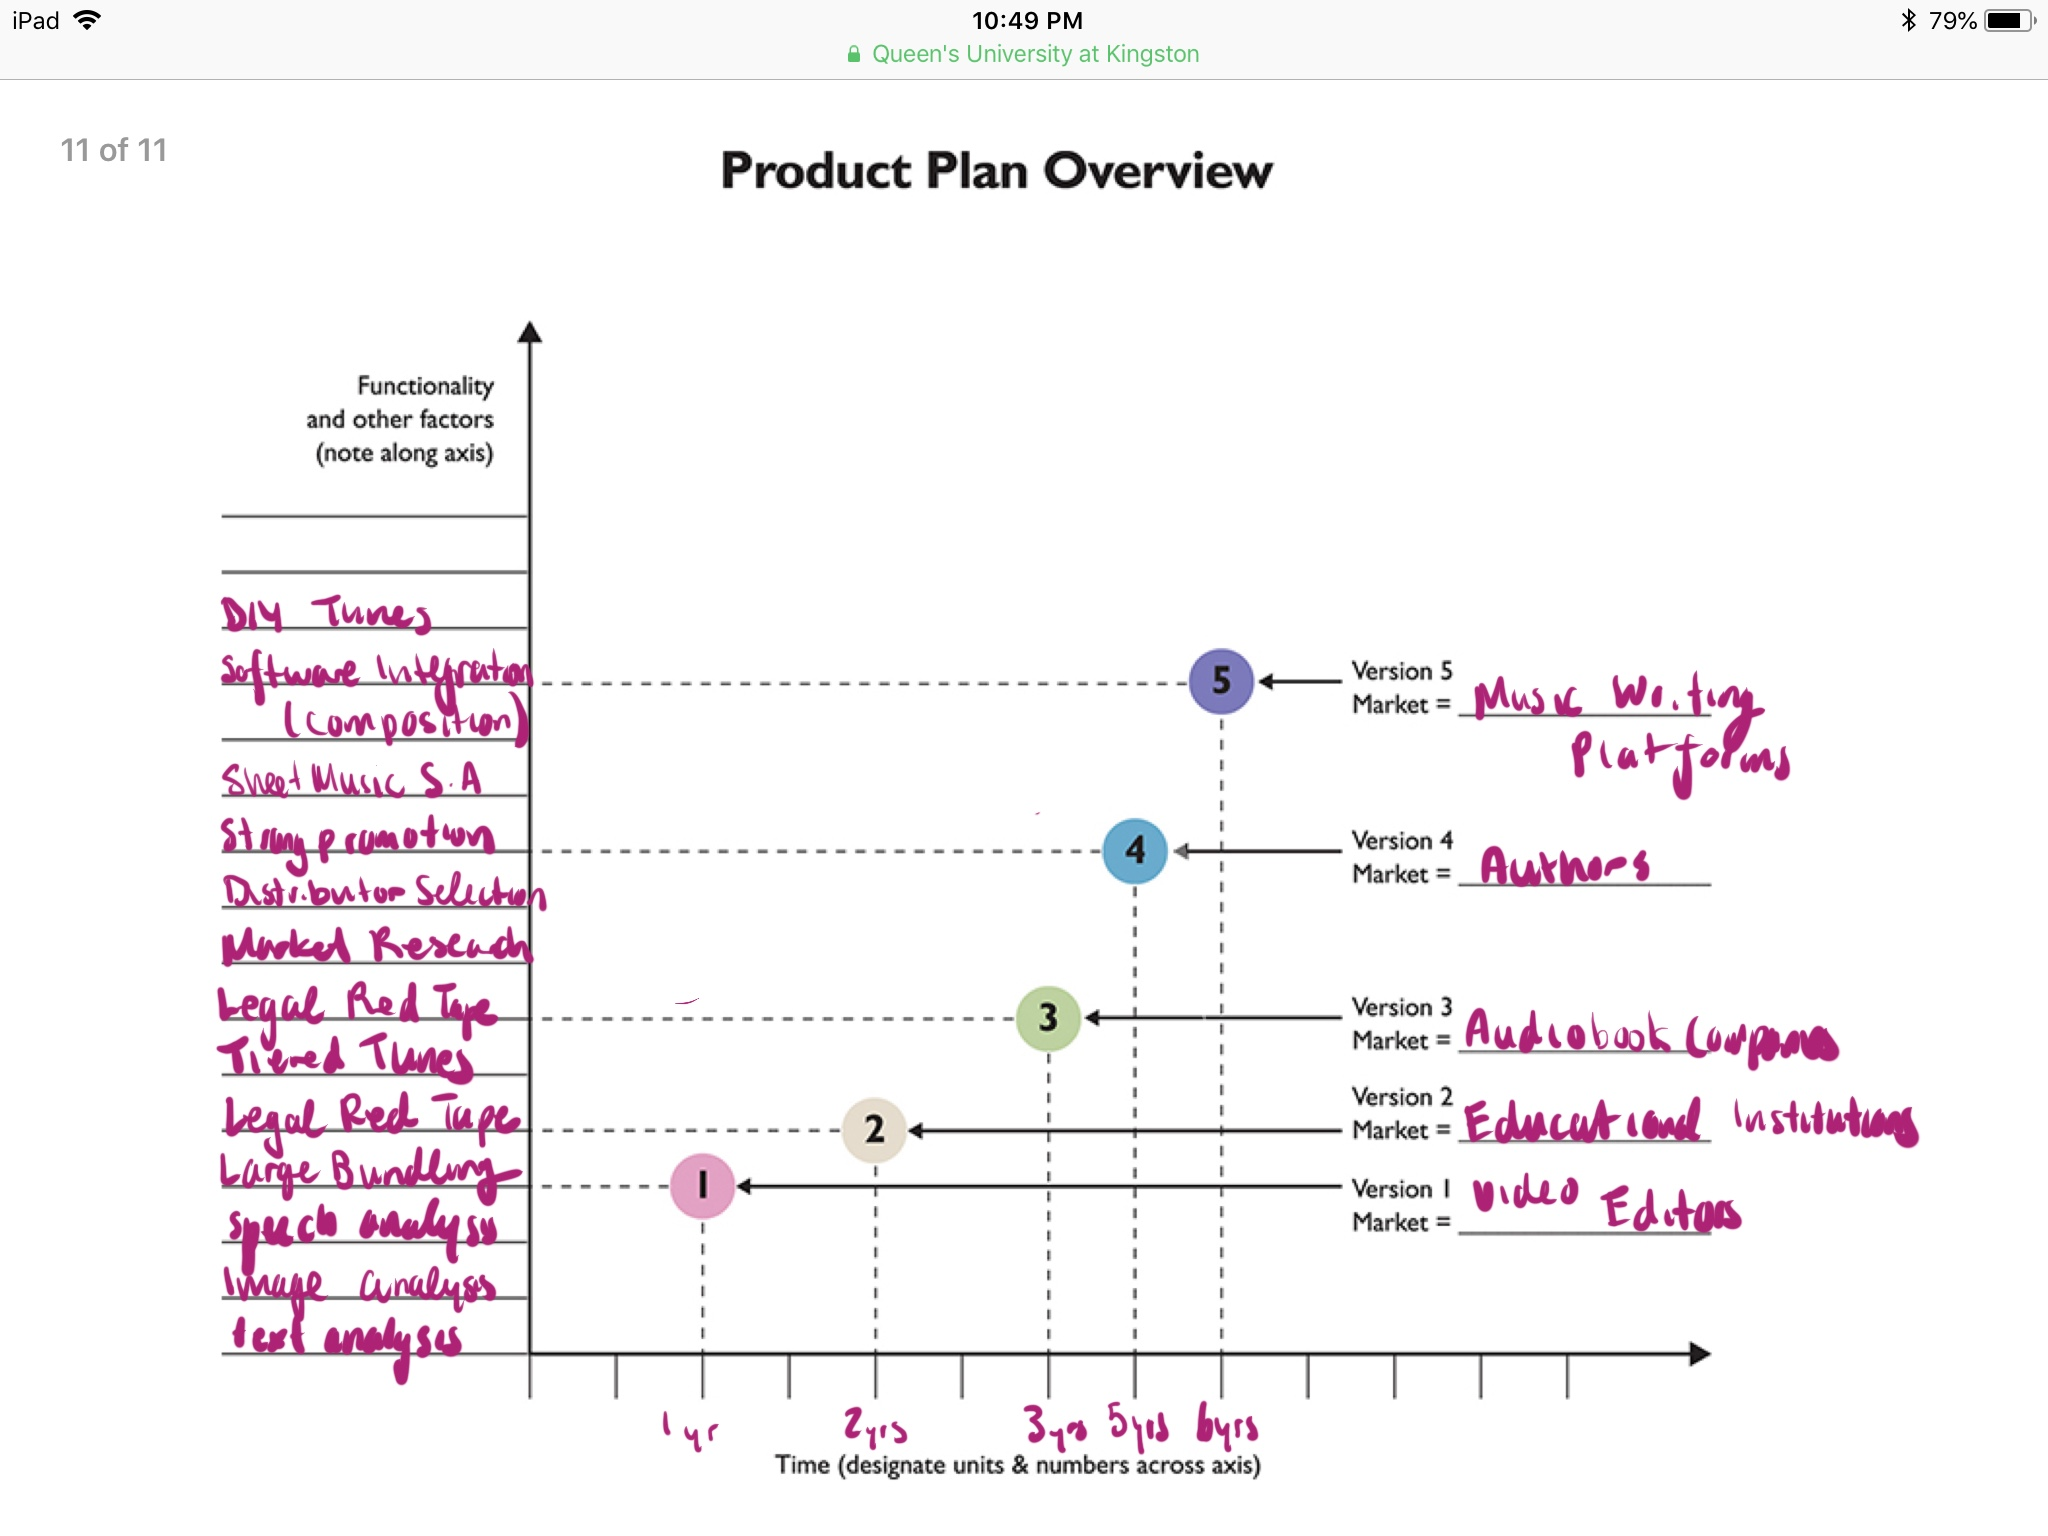
\includegraphics[width=15cm,height=10cm]{ProductPlan}
            \caption{Image detailing the product plan overview. Due to technical issues it could not be cropped properly.}
        \end{center}
    \end{figure}

    \cleardoublepage

    \section{References}
    \begin{itemize}
        \item Aha! Labs. (n.d.). A complete guide to product roadmaps (with examples). Aha! Retrieved February 22, 2021, from \url{https://www.aha.io/roadmapping/guide/product-roadmap}
        \item Ashtikar, M. (2020, September 1). 4 drivers for increasing customer lifetime value for field service businesses. Acrotrend Solutions. \url{https://www.acrotrend.com/4-vital-clv-drivers-for-field-service-management-businesses/}
        \item Aulet, B. (2013). Disciplined Entrepreneurship: 24 Steps to a Successful Startup (1st ed.). Wiley. \url{https://ocul-qu.primo.exlibrisgroup.com/discovery/fulldisplay?context=L&vid=01OCUL_QU:QU_DEFAULT&search_scope=OCULDiscoveryNetwork&tab=OCULDiscoveryNetwork&docid=alma991715536305151}
        \item Brown, J. (2018, December 1). How Much Should Your SaaS Marketing Budget Be? - Big Drop Inc Blog. Big Drop Inc. \url{https://www.bigdropinc.com/blog/how-much-should-your-saas-marketing-budget-be/#:%7E:text=According%20to%20OpenView’s%202017%20Benchmarks,the%20life%20of%20the%20company.}
        \item Coffey, B. (2013, July 9). SaaS Unit Economics - Calculating COCA by Segment (and why its hard). BradfordCoffrey.Com. \url{://www.bradfordcoffey.com/blog/bid/56074/saas-unit-economics-calculating-coca-by-segment-and-why-its-hard#:%7E:text=At%20a%20high%20level%20calculating,customers%20acquired%20in%20the%20period.}
        \item Cook, D. (2020, October). Design, Editing \& Rendering Software Publishing in the US. Ibisworld. \url{https://my-ibisworld-com.proxy.queensu.ca/us/en/industry/51121d/industry-at-a-glanceDan, K. (2020, July 6). How Much Do Audiobook Narrators Make? Naturally Voice | Every Voice Has a Story to Tell! https://naturallyvoice.com/how-much-do-audiobook-narrators-make/}
        \item Koronios, E. (2020, December). Book Publishing in Canada. Ibisworld. \url{https://login.proxy.queensu.ca/login?qurl=https://my.ibisworld.com%2fca%2fen%2findustry%2f51113ca%2findustry-at-a-glance}
        \item Masters, N. (2019, December). Audiobook Publishing in the US.Ibisworld. \url{https://login.proxy.queensu.ca/login?qurl=https://my.ibisworld.com%2fus%2fen%2findustry-specialized%2fod4396%2findustry-at-a-glanceO’Connor, C. (2020, September). Online Tutoring Services. Ibisworld. https://my-ibisworld-com.proxy.queensu.ca/us/en/industry-specialized/od6038/industry-at-a-glance}
        \item Rodriguez, A. (2019, September). Sheet Music Publishers. Ibisworld. \url{https://login.proxy.queensu.ca/login?qurl=https://my.ibisworld.com%2fus%2fen%2findustry-specialized%2fod4845%2findustry-at-a-glanceSmyth, D. (2020, November 10). How Do Publishers Get Royalties for Audio Books? Work - Chron.Com. https://work.chron.com/publishers-royalties-audio-books-14264.html}
        \item Staff, C. B. (2021, January 21). Best video editing software: Top tools in 2021. Creative Bloq. \url{https://www.creativebloq.com/features/best-video-editing-software-for-designers}
        \item Wascher, K. (2020, February 12). How much does it cost to record an audiobook? Krystal Wascher. \url{https://krystalwascher.com/blog-audiobooks-for-authors/how-much-does-it-cost-to-create-an-audiobook}
    \end{itemize}
\end{document}